Both a parameterized and an unparameterized model were used to classify potential sites of metabolism.
IDSite makes the assumptions that all intermediates before the rate determining step are at equilibrium \cite{wang2007stochastic}, that hydrogen abstraction is the rate limiting step for hydroxilation of aliphatic carbons and electrophilic attack is the rate limiting step for hydroxilation of aromatic rings \cite{guengerich2001common,shaik2005theoretical}.
With these assumptions the rate of metabolism at each possible site of reaction is affected by the free energy of binding in order to put that site in the site of reaction, as well as the free energy barrier of rate determining step, or
\begin{equation}
{\Delta}G_{\mathrm{total}} = {\Delta}G_{\mathrm{binding}} + {\Delta}G_{\mathrm{barrier}}
\end{equation}
 % dG = dG bind + dG react
The ${\Delta}G_{\mathrm{binding}}$ above is calculated using a PLOP evaluation of the refined pose.
The intrinsic reactivity for the system is computed from DFT calculations on a simplified system, replacing the heme with a methody radical, and using a linear relationship between $IR(\mathrm{heme})$ and $IR(\mathrm{methoxy\ radical})$ to estimate the true reactivity for the heme system.
\begin{figure}[h]
\centering
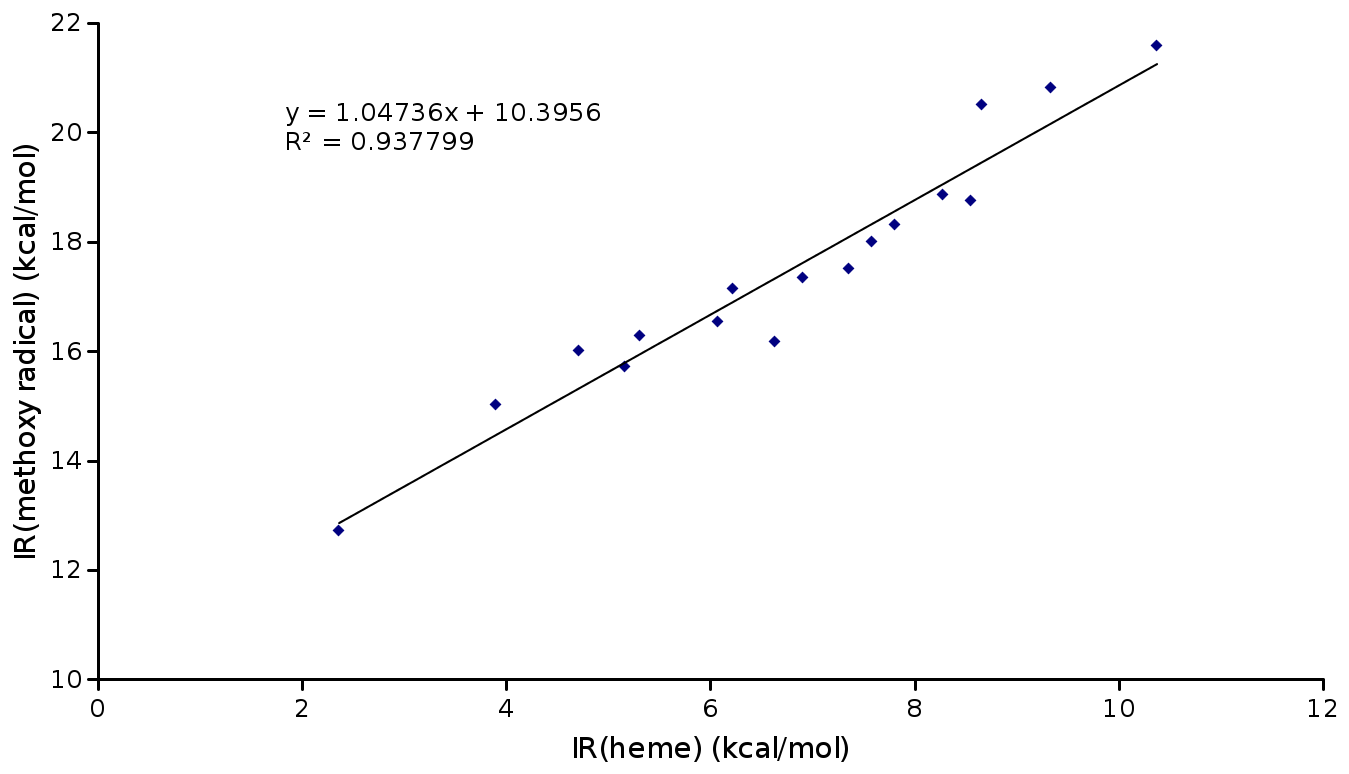
\includegraphics[width=0.8\textwidth]{figures/idsite/intrinsic_corrected.png}
\caption{The linear relationship between the calculated intrinsic reactivity of the methoxy radical complex and that of the heme complex.
Adapted from \protect\cite{li2011idsite} with minor correction.
In the original manuscript the slope of the regression was reported as 1.117 and that number was used throughout.
This difference should not significantly affect the physical IDSite classifier results, and does not affect the results of the fit model.
In the rest of this text the value from the original publication of 1.117 will be used.}
\label{fig:idsite/intrinsic}
\end{figure}
\begin{table}[h]
\centering
\label{table:heme_methoxy}
\begin{tabular}{cccc}
\hline
Model compound & Site of Metabolism & Heme model (kcal/mol) & Methoxy model (kcal/mol) \\
\hline
Benzene &  & 20.51 & 8.66 \\
Anisole & Ortho- & 16.29 & 5.31 \\
 & Meta- & 18.76 & 8.55 \\
 & Para- & 16.01 & 4.71 \\
 & Beta- & 16.18 & 6.63 \\
Dimethylether &  & 15.03 & 3.9 \\
Dimethylanisole & Meta- & 16.54 & 6.07 \\
 & Para- & 17.51 & 7.35 \\
Ethane &  & 21.58 & 10.37 \\
Ethanol & 1 & 12.73 & 2.36 \\
 & 2 & 17.35 & 6.9 \\
Propane &  & 18.31 & 7.8 \\
Toluene & Ortho- & 17.15 & 6.22 \\
 & Meta- & 18.86 & 8.27 \\
 & Para- & 18 & 7.58 \\
 & Alpha- & 15.72 & 5.16 \\
t-Butylebenzene & Beta- & 20.82 & 9.33 \\
\hline
\end{tabular}
\caption{DFT calculated values for internal reactivity of various compounds with either methoxy radical (compound I) or heme system.
Correlation between these values is illustrated in Figure \ref{fig:idsite/intrinsic}.}
\end{table}

\begin{equation}
\mathrm{IR}(\mathrm{heme}) = 1.117 * \mathrm{IR}(\mathrm{methoxy\ radical}) + C
\end{equation}
 % estimate from abbreviated reactivity
Since this constant $C$ is identical for each state it has no effect on the relative differences in ${\Delta}G_{\mathrm{site}}$ or the relative rate of metabolism at possible sites.
\begin{equation}
\label{equation:g_site}
E = \langle 1.117 * \mathrm{IR}(\mathrm{methoxyradical}) + C + E_{\mathrm{TS}} \rangle - kT\ ln(N_H)
\end{equation}
 % E/G equation
Since the ligand is forced to assume a different conformation in order to react, the energy of this transition state conformation, $E_{\mathrm{TS}}$, is also computed using PLOP.
As the relative abundance of different metabolites is determined by differences in ${\Delta}G$ per site rather than absolute reactivities, the constant in equation \ref{equation:g_site} does not affect which metabolites are produced.
A site of possible metabolism is classified as positive if it is observed in greater than 0.1\% yield, which corresponds to a \ddg\ of \textapprox4.75 kcal/mol between the most favored state and the cutoff for negative predictions. 

The second classifier is similar however:
\begin{enumerate}
\item a different constant is used to estimate $IR(\mathrm{heme})$ from $IR(\mathrm{methoxy\ radical})$, namely 1.071,
\item if the binding energy of the transition state complex of a pose is within 5.26 kcal/mol of the lowest pose, it is set to the binding energy of the lowest pose.
Otherwise the difference is scaled by 0.58,
\item and the cutoff for an active prediction is changed from 4.75 kcal/mol to 1.46 kcal/mol.
\end{enumerate}
These parameters were decided upon by maximizing $\frac{\mathrm{true\ positives}}{(\mathrm{false\ positives + false\ negatives})}$ on a training set of 36 compounds.
